\documentclass[12pt,a4paper,oneside]{report}

\usepackage[utf8]{inputenc}
\usepackage[T1]{fontenc}
% Label berbahasa Indonesia (mandiri tanpa ketergantungan paket babel-indonesian)
\renewcommand{\chaptername}{BAB}
\renewcommand{\contentsname}{DAFTAR ISI}
\renewcommand{\listtablename}{DAFTAR TABEL}
\renewcommand{\listfigurename}{DAFTAR GAMBAR}
\renewcommand{\bibname}{DAFTAR PUSTAKA}
\renewcommand{\tablename}{Tabel}
\renewcommand{\figurename}{Gambar}
\usepackage{mathptmx}
\usepackage{courier}
\usepackage{microtype}
\usepackage{xurl}
\usepackage{geometry}
\geometry{left=4cm,top=3cm,right=3cm,bottom=3cm}
\usepackage{setspace}
\onehalfspacing

\usepackage{graphicx}
\usepackage{booktabs}
\usepackage{longtable}
\usepackage{array}
\usepackage{float}
\usepackage{enumitem}
\usepackage{xcolor}
\usepackage{listings}
\usepackage{caption}
\usepackage{titlesec}
\usepackage[hidelinks]{hyperref}

% Format judul bab bergaya laporan akademik Indonesia
\titleformat{\chapter}[display]
  {\normalfont\bfseries\centering\fontsize{14}{17}\selectfont}
  {\MakeUppercase{\chaptertitlename}\ \thechapter}{0.5em}{\MakeUppercase}
\titlespacing*{\chapter}{0pt}{-15pt}{18pt}

\titleformat{\section}
  {\normalfont\bfseries\fontsize{12}{15}\selectfont}{\thesection}{1em}{}
\titleformat{\subsection}
  {\normalfont\bfseries\fontsize{12}{15}\selectfont}{\thesubsection}{1em}{}

% Gaya cuplikan kode sumber
\lstset{
  basicstyle=\ttfamily\footnotesize,
  breaklines=true,
  frame=single,
  rulecolor=\color{gray!40},
  backgroundcolor=\color{gray!5},
  numbers=left,
  numberstyle=\tiny\color{gray},
  captionpos=b
}

% =========================================================================
% KONFIGURASI METADATA LAPORAN PROYEK 2 CONECKIN
% Ubah nilai [ISI ...] sesuai data lengkap kelompok dan dosen pembimbing.
% =========================================================================
\newcommand{\JudulLaporan}{Pengembangan, Pengujian Otomatis, dan Integrasi Ekosistem Aplikasi Coneckin Berbasis Arsitektur Hybrid CRUD untuk Otomasi Login Captive Portal WiFi Kampus}
\newcommand{\JudulInggris}{Development, Automated Testing, and Ecosystem Integration of Coneckin Application Based on Hybrid CRUD Architecture for Campus WiFi Captive Portal Login Automation}

\newcommand{\NamaPenulisSatu}{Muhammad Aris Ashidiqi}
\newcommand{\NimPenulisSatu}{714250042}

% Apabila proyek dikerjakan berkelompok, isi anggota kedua di bawah ini.
% Jika dikerjakan individu, kosongkan teks di dalam kurung kurawal.
\newcommand{\NamaPenulisDua}{[ISI NAMA ANGGOTA 2 / KOSONGKAN JIKA INDIVIDU]}
\newcommand{\NimPenulisDua}{[ISI NIM ANGGOTA 2]}

\newcommand{\NamaDosenPembimbing}{[ISI NAMA DOSEN PEMBIMBING \& GELAR]}
\newcommand{\NidnDosenPembimbing}{[ISI NIDN/NIK DOSEN]}

\newcommand{\NamaProdi}{D4 Teknik Informatika}
\newcommand{\NamaFakultas}{Sekolah Vokasi}
\newcommand{\NamaUniversitas}{Universitas Logistik dan Bisnis Internasional (ULBI)}
\newcommand{\KotaKampus}{Bandung}
\newcommand{\TahunLaporan}{2026}


\begin{document}
\sloppy

% ---------- Bagian Awal (Romawi) ----------
\pagenumbering{roman}
% ---------- HALAMAN SAMPUL ----------
\begin{titlepage}
\begin{center}
\textbf{\large LAPORAN PROYEK 2}\\[1.2cm]

\textbf{\Large \MakeUppercase{\JudulLaporan}}\\[1.5cm]

% Jika sudah menambahkan logo ULBI di images/logo-ulbi.png, hapus tanda % di bawah:
% 
\includegraphics[width=4.2cm]{images/logo-ulbi.png}\\[1.5cm]

Disusun untuk Memenuhi Tugas Mata Kuliah Proyek 2\\
Program Studi \NamaProdi\\[1.5cm]

\textbf{Disusun Oleh:}\\[0.4cm]
\begin{tabular}{ll}
\NamaPenulisSatu & (\NimPenulisSatu) \\
\NamaPenulisDua & (\NimPenulisDua) \\
\end{tabular}\\[1.8cm]

\textbf{Dosen Pembimbing:}\\
\NamaDosenPembimbing\\
NIDN/NIK: \NidnDosenPembimbing\\[2cm]

\vfill
\textbf{\MakeUppercase{Program Studi \NamaProdi}}\\
\textbf{\MakeUppercase{\NamaFakultas}}\\
\textbf{\MakeUppercase{\NamaUniversitas}}\\
\textbf{\MakeUppercase{\KotaKampus}}\\
\textbf{\TahunLaporan}
\end{center}
\end{titlepage}

% ---------- ABSTRAK (INDONESIA) ----------
\chapter*{ABSTRAK}
\addcontentsline{toc}{chapter}{ABSTRAK}

Jaringan WiFi kampus umumnya menggunakan mekanisme \textit{captive portal} berbasis web yang mengharuskan pengguna memasukkan kredensial secara berulang setiap kali sesi terputus atau perangkat berpindah titik akses. Proyek 2 ini mengembangkan, melengkapi, dan memverifikasi ekosistem aplikasi \textbf{Coneckin} yang terdiri atas aplikasi Android native berbasis Kotlin dan Jetpack Compose, layanan API REST berbasis Node.js (Express 5) dan MongoDB (\texttt{coneckin\_db}), serta halaman panduan dan unduhan berbasis konvensi modular Croot.js pada GitHub Pages (\texttt{coneckin.github.io}).

Penyempurnaan utama mencakup pemenuhan arsitektur \textit{Hybrid CRUD} secara utuh melalui penambahan fitur \textit{Ubah Akun} pada sisi penyimpanan lokal terenkripsi AES-256 GCM (\texttt{AndroidKeyStore}) serta implementasi operasi \textit{Create}, \textit{Read}, \textit{Update}, dan \textit{Delete} pada endpoint server (\texttt{/portals}, \texttt{/config}, \texttt{/reports}) yang dilindungi autentikasi token admin berbasis perbandingan aman waktu-konstan (SHA-256 \texttt{timingSafeEqual}) dan middleware CORS untuk endpoint baca publik. Dari sisi penjaminan mutu, diterapkan pengujian otomatis berlapis dengan hasil 78 \textit{unit test} JVM Android dengan \textit{line coverage} 95,80\%, 11 \textit{instrumented test} perangkat Android untuk validasi \texttt{AndroidKeyStore}, serta 39 tes otomatis pada server Express dengan \textit{line coverage} 96,53\%. Seluruh pengujian terintegrasi dalam alur CI/CD GitHub Actions yang mensyaratkan ambang \textit{coverage} minimal 80\% sebelum merilis APK dan AAB, serta telah tervalidasi berjalan sinkron di lingkungan produksi Alwaysdata dan GitHub Pages.

\vspace{0.5cm}
\noindent\textbf{Kata Kunci:} Captive Portal, Hybrid CRUD, Android Kotlin, AES-256 GCM, Code Coverage, Croot.js.

\clearpage

% ---------- ABSTRACT (ENGLISH) ----------
\chapter*{ABSTRACT}
\addcontentsline{toc}{chapter}{ABSTRACT}

Campus WiFi networks commonly rely on web-based captive portals that require users to repeatedly enter their credentials whenever sessions expire or devices roam across access points. This Project 2 develops, completes, and verifies the \textbf{Coneckin} ecosystem, consisting of a native Android application built with Kotlin and Jetpack Compose, a Node.js (Express 5) and MongoDB (\texttt{coneckin\_db}) REST API service, and a Croot.js-based landing page hosted on GitHub Pages (\texttt{coneckin.github.io}).

Core enhancements complete the Hybrid CRUD architecture by adding an account editing feature (\textit{Ubah Akun}) backed by local AES-256 GCM encryption (\texttt{AndroidKeyStore}), alongside full administrative CRUD endpoints (\texttt{/portals}, \texttt{/config}, \texttt{/reports}) protected by constant-time SHA-256 token verification (\texttt{timingSafeEqual}) and public read CORS support. Multi-layered automated testing achieves 78 Android JVM unit tests with 95.80\% line coverage, 11 Android instrumented tests validating \texttt{AndroidKeyStore} operations on an emulator, and 39 Express API tests reaching 96.53\% line coverage. All test suites are enforced inside GitHub Actions CI/CD pipelines requiring at least 80\% line coverage prior to automated APK/AAB releases, and have been verified end-to-end across Alwaysdata production hosting and GitHub Pages.

\vspace{0.5cm}
\noindent\textbf{Keywords:} Captive Portal, Hybrid CRUD, Android Kotlin, AES-256 GCM, Code Coverage, Croot.js.

\clearpage

% ---------- KATA PENGANTAR ----------
\chapter*{KATA PENGANTAR}
\addcontentsline{toc}{chapter}{KATA PENGANTAR}

Puji syukur penulis panjatkan ke hadirat Tuhan Yang Maha Esa atas rahmat dan karunia-Nya sehingga laporan Proyek 2 dengan judul \textit{\JudulLaporan} dapat diselesaikan tepat waktu. Laporan ini disusun sebagai bagian dari luaran akademik mata kuliah Proyek 2 pada Program Studi \NamaProdi, \NamaUniversitas.

Penulis menyampaikan terima kasih kepada \NamaDosenPembimbing\ selaku dosen pembimbing yang telah memberikan arahan selama proses analisis, implementasi, pengujian, dan penyusunan dokumentasi ekosistem Coneckin. Penulis menyadari bahwa laporan ini masih terbuka terhadap saran dan penyempurnaan. Semoga dokumentasi dan perangkat lunak yang dihasilkan dapat memberikan manfaat nyata bagi sivitas akademika maupun pengembang selanjutnya.

\vspace{1cm}
\begin{flushright}
\KotaKampus, November \TahunLaporan\\[1.5cm]
Penulis
\end{flushright}
\clearpage


\tableofcontents
\clearpage
\listoftables
\clearpage
\listoffigures
\clearpage

% ---------- Bagian Isi (Arab) ----------
\pagenumbering{arabic}
\chapter{Pendahuluan}

\section{Latar Belakang}
Layanan jaringan nirkabel (WiFi) di lingkungan perguruan tinggi umumnya dilindungi mekanisme \textit{captive portal} berbasis web agar hanya sivitas akademika yang memiliki akun resmi yang dapat mengakses internet \cite{rfc8952}. Kendati efektif dari sisi pengendalian akses, proses autentikasi manual melalui peramban menimbulkan friksi ketika pengguna berpindah gedung, sesi kedaluwarsa, atau perangkat terputus sementara dari titik akses (\textit{access point}). Pengguna harus membuka ulang halaman portal dan mengetikkan nama pengguna serta kata sandi secara berulang.

Aplikasi \textbf{Coneckin} hadir sebagai solusi Android native berbasis Kotlin dan Jetpack Compose yang memungkinkan proses masuk ke portal WiFi kampus cukup dengan satu ketukan, baik dari layar utama aplikasi maupun lewat \textit{Quick Settings Tile}. Untuk menjaga privasi, kredensial pengguna disimpan terenkripsi lokal di perangkat memakai AES-256 GCM melalui \texttt{AndroidKeyStore} tanpa pernah dikirim ke server pusat \cite{android_keystore,nist_gcm}. Sementara itu, layanan server REST API pada Node.js dan MongoDB menyediakan direktori portal kampus terverifikasi, informasi konfigurasi rilis aplikasi, dan penampung laporan gangguan anonim bersifat opsional (\textit{opt-in}).

Pada versi awal aplikasi, masih terdapat beberapa kesenjangan rekayasa perangkat lunak yang perlu diselesaikan dalam Proyek 2:
\begin{enumerate}[leftmargin=*]
  \item Operasi \textit{Update} pada penyimpanan akun lokal Android belum tersedia sehingga pengguna harus menghapus dan membuat ulang akun ketika kata sandi atau alamat portal berubah.
  \item Layanan server API sebelumnya baru menyediakan operasi baca publik (\texttt{GET /portals}, \texttt{GET /config}) dan tambah laporan (\texttt{POST /reports}), belum memiliki endpoint CRUD administratif lengkap maupun header CORS bagi konsumsi web.
  \item Pengujian otomatis belum mencakup pengukuran \textit{code coverage}, belum menyertakan pengujian instrumentasi untuk \texttt{AndroidKeyStore}, dan alur CI GitHub Actions belum menegakkan ambang kelulusan uji sebelum membangun rilis APK/AAB.
  \item Belum tersedianya halaman panduan dan direktori portal berbasis konvensi modular Croot.js pada repositori terpisah \texttt{coneckin.github.io} yang tersinkronisasi langsung dengan API produksi dan rilis APK terbaru.
\end{enumerate}

\section{Rumusan Masalah}
Berdasarkan latar belakang tersebut, rumusan masalah pada Proyek 2 ini adalah sebagai berikut:
\begin{enumerate}[leftmargin=*]
  \item Bagaimana merancang dan melengkapi arsitektur \textit{Hybrid CRUD} secara penuh pada sisi penyimpanan terenkripsi lokal Android serta pada layanan REST API server MongoDB?
  \item Bagaimana menerapkan mekanisme penjaminan mutu berbasis pengujian otomatis (\textit{unit test}, \textit{instrumented test}, dan pengujian integrasi API) dengan ambang \textit{line coverage} minimal 80\% yang terintegrasi dalam pipeline CI/CD?
  \item Bagaimana membangun \textit{landing page} panduan instalasi dan direktori portal berbasis konvensi Croot.js pada \texttt{coneckin.github.io} yang terhubung langsung ke API produksi dan rilis APK terbaru?
  \item Bagaimana mengotomatisasi penyusunan dan rilis dokumentasi akademik LaTeX pada repositori organisasi GitHub Coneckin?
\end{enumerate}

\section{Tujuan Proyek}
Tujuan yang dicapai dalam pelaksanaan Proyek 2 ini meliputi:
\begin{enumerate}[leftmargin=*]
  \item Melengkapi fitur \textit{Ubah Akun} pada aplikasi Android Coneckin serta memisahkan logika bisnis murni agar dapat diuji pada JVM tanpa ketergantungan antarmuka.
  \item Mengimplementasikan endpoint CRUD lengkap pada server Express 5 dan MongoDB (\texttt{coneckin\_db}) yang diamankan otorisasi token admin (SHA-256 \texttt{timingSafeEqual}) serta CORS baca publik.
  \item Mencapai \textit{code coverage} $\ge 80\%$ pada lapisan logika Android (JaCoCo) dan server Node.js, dilengkapi \textit{instrumented test} \texttt{AndroidKeyStore} dan integrasi \textit{test-before-release} di GitHub Actions.
  \item Menayangkan \textit{landing page} responsif berbasis konvensi Croot.js di \url{https://coneckin.github.io/} yang terhubung langsung dengan API produksi di \url{https://panlink.alwaysdata.net}.
  \item Menyediakan alur kompilasi dan rilis otomatis dokumen PDF berbasis LaTeX pada repositori \texttt{laporan} dan \texttt{jurnal}.
\end{enumerate}

\section{Ruang Lingkup dan Struktur Ekosistem}
Ekosistem Coneckin dikelola pada organisasi GitHub \url{https://github.com/coneckin} yang terbagi ke dalam lima repositori resmi sebagaimana dirangkum pada Tabel~\ref{tab:ekosistem}.

\begin{table}[H]
\centering
\caption{Pemetaan Lima Repositori Ekosistem Proyek 2 Coneckin}
\label{tab:ekosistem}
\begin{tabular}{@{}p{3.1cm}p{4.1cm}p{5.6cm}@{}}
\toprule
\textbf{Repositori} & \textbf{Teknologi Utama} & \textbf{Peran dalam Ekosistem} \\
\midrule
\texttt{coneckin} & Kotlin, Jetpack Compose, JUnit 4, JaCoCo; Node.js, Express 5, MongoDB & Aplikasi Android native, API server REST, pengujian otomatis, dan CI/CD rilis APK/AAB. \\
\texttt{coneckin.github.io} & HTML5, CSS3, ES6 Module (konvensi Croot.js) & \textit{Landing page} panduan instalasi, direktori portal dinamis, status API, dan tautan rilis APK terbaru. \\
\texttt{laporan} & LaTeX, GitHub Actions & Laporan akhir Proyek 2 dengan kompilasi dan rilis PDF otomatis. \\
\texttt{jurnal} & LaTeX, GitHub Actions & Artikel ilmiah Proyek 2 dalam format jurnal dengan rilis PDF otomatis. \\
\texttt{presentasi} & Crootss.if.co.id & Dek slide presentasi untuk demo dan sidang Proyek 2. \\
\bottomrule
\end{tabular}
\end{table}

\section{Sistematika Penulisan}
Laporan ini disusun dalam lima bab: Bab~1 membahas latar belakang, rumusan masalah, tujuan, dan ruang lingkup; Bab~2 menguraikan landasan teori dan teknologi yang digunakan; Bab~3 menjelaskan analisis arsitektur \textit{Hybrid CRUD}, keamanan, dan perancangan sistem; Bab~4 memaparkan hasil implementasi, pengujian otomatis, dan verifikasi produksi; serta Bab~5 berisi kesimpulan dan saran pengembangan lanjutan.

\chapter{Tinjauan Pustaka}

\section{Arsitektur Captive Portal WiFi}
\textit{Captive portal} merupakan mekanisme pengalihan lalu lintas jaringan yang menahan akses internet klien baru hingga proses autentikasi atau persetujuan kebijakan selesai dilakukan melalui halaman web portal \cite{rfc8952}. Pada Android 10 (API 29) ke atas, sistem operasi mendeteksi kondisi portal secara otomatis dan menandai jaringan WiFi tanpa akses internet sampai halaman login diselesaikan. Otomasi login pada sisi klien harus memperhatikan pencocokan nama host secara ketat agar kredensial tidak pernah disuntikkan ke halaman pihak ketiga yang tidak sah.

\section{Arsitektur Hybrid CRUD}
Dalam aplikasi seluler berorientasi privasi, pemisahan lokasi penyimpanan data sangat krusial. Pendekatan \textit{Hybrid CRUD} membagi siklus hidup data ke dua lapisan terpisah:
\begin{itemize}[leftmargin=*]
  \item \textbf{CRUD Lokal Terenkripsi (Sisi Perangkat):} Data sensitif milik pengguna (daftar akun portal, username, password, dan daftar host) dikelola penuh di perangkat melalui operasi \textit{Create}, \textit{Read}, \textit{Update}, dan \textit{Delete} tanpa sinkronisasi ke cloud.
  \item \textbf{CRUD Terpusat (Sisi Server API):} Data referensi publik dan operasional non-pribadi—yakni direktori portal kampus (\texttt{portals}), konfigurasi versi dan pengumuman (\texttt{app\_config}), serta laporan gangguan anonim (\texttt{reports})—dikelola di server basis data MongoDB \cite{mongodb_node} melalui REST API Express 5 \cite{express_docs}.
\end{itemize}

\section{Enkripsi AES-256 GCM dan Android Keystore}
\textit{Advanced Encryption Standard} dengan mode \textit{Galois/Counter Mode} (AES-256 GCM) menyediakan enkripsi terautentikasi (\textit{authenticated encryption}) yang menjamin kerahasiaan sekaligus integritas \textit{ciphertext} menggunakan \textit{Initialization Vector} (IV) unik dan tag autentikasi \cite{nist_gcm}. Pada platform Android, penyimpanan kunci kriptografi di \texttt{AndroidKeyStore} melindungi materi kunci agar tidak mudah diekstraksi dari ruang proses aplikasi maupun ikut tersalin saat pencadangan sistem \cite{android_keystore}.

\section{Konvensi Modular Croot.js}
Croot.js memperkenalkan pendekatan pengembangan antarmuka web statis berbasis modul ECMAScript (ES6 Modules) tanpa ketergantungan \textit{bundler} berat \cite{crootjs_repo}. Struktur kode dipisahkan secara bersih ke dalam direktori konfigurasi (\texttt{js/config/}), pustaka utilitas (\texttt{js/lib/}), pengontrol logika halaman (\texttt{js/controller/}), dan satu titik masuk utama (\texttt{js/croot.js}), sehingga sangat cocok diterapkan pada layanan hosting statis seperti GitHub Pages.

\section{Pengujian Otomatis, Code Coverage, dan CI/CD}
Penjaminan mutu perangkat lunak modern memadukan pengujian unit cepat pada JVM/Node.js, pengujian instrumentasi pada lingkungan perangkat nyata atau emulator, serta pengukuran \textit{code coverage} untuk mengidentifikasi cabang logika yang belum teruji. Pada ekosistem Android/JVM, \textbf{JaCoCo} mengukur cakupan baris dan cabang secara deterministik \cite{jacoco_docs}, sedangkan pada Node.js versi 20 ke atas tersedia \textit{built-in test runner} beserta bendera \texttt{--experimental-test-coverage} yang memungkinkan penegakan ambang \textit{coverage} langsung tanpa pustaka tambahan \cite{nodejs_test_runner}. Integrasi pada GitHub Actions memastikan setiap perubahan yang masuk ke cabang utama (\texttt{main}) telah lulus seluruh rangkaian tes sebelum paket rilis diterbitkan.

\chapter{Analisis dan Perancangan Sistem}

\section{Arsitektur Sistem Terintegrasi}
Ekosistem Coneckin menerapkan arsitektur tiga lapis yang saling terhubung melalui protokol HTTPS:
\begin{enumerate}[leftmargin=*]
  \item \textbf{Klien Android (\texttt{coneckin/app}):} Menyimpan kredensial akun terenkripsi lokal (AES-256 GCM), menjalankan deteksi portal dan otomasi login di latar belakang melalui WebView dengan validasi host ketat, menyediakan \textit{Quick Settings Tile} (\texttt{LoginTileService}), kunci perangkat (\texttt{AppLock}), serta menyinkronkan direktori portal dan konfigurasi versi dari server API.
  \item \textbf{Layanan Server API (\texttt{coneckin/server}):} Berjalan pada Node.js dengan Express 5 di hosting Alwaysdata (\url{https://panlink.alwaysdata.net}) dan basis data MongoDB (\texttt{coneckin\_db}). Lapisan logika murni (\texttt{lib.js}) dan definisi aplikasi (\texttt{app.js}) dipisahkan dari \textit{bootstrap} jaringan (\texttt{server.js}) agar seluruh endpoint dapat diuji secara terisolasi.
  \item \textbf{Antarmuka Web (\texttt{coneckin.github.io}):} Halaman statis berbasis ES6 Module (konvensi Croot.js) di GitHub Pages yang mengonsumsi endpoint publik \texttt{GET /config}, \texttt{GET /portals}, dan \texttt{GET /health}, sekaligus menautkan tombol unduhan langsung ke aset \texttt{coneckin.apk} pada GitHub Releases terbaru.
\end{enumerate}

\section{Perancangan Hybrid CRUD}
\subsection{CRUD Lokal Android}
Untuk melengkapi siklus CRUD pada penyimpanan akun lokal sekaligus menjaga agar logika bisnis dapat diuji pada JVM, fungsi pengelolaan akun dipecah ke dalam modul \texttt{AccountRepository} dan \texttt{AccountOps} di atas lapisan penyimpanan terenkripsi \texttt{AccountStore} dan \texttt{CryptoManager}:
\begin{itemize}[leftmargin=*]
  \item \textbf{Create:} Menambahkan akun baru dengan validasi nama, username, password, dan normalisasi daftar alamat host portal.
  \item \textbf{Read:} Memuat daftar akun tersimpan, menentukan akun aktif terpilih, serta menampilkan daftar portal dari cache lokal atau server.
  \item \textbf{Update (Fitur Baru Proyek 2):} Memungkinkan pengguna menyunting nama akun, kredensial, dan daftar portal pada akun yang sudah ada melalui dialog \textit{Ubah Akun} tanpa kehilangan status akun aktif.
  \item \textbf{Delete:} Menghapus akun tertentu beserta penyesuaian otomatis pemilihan akun aktif bila akun yang dihapus sedang aktif.
\end{itemize}

\subsection{CRUD Server API (\texttt{coneckin\_db})}
Basis data \texttt{coneckin\_db} terdiri atas tiga koleksi utama: \texttt{portals} (indeks unik pada field \texttt{host}, data awal \texttt{ULBI — ypbpi.hotspot}), \texttt{app\_config} (dokumen tunggal \texttt{\_id: "main"}), dan \texttt{reports} (indeks TTL otomatis 90 hari atau 7.776.000 detik dengan batas maksimum 20.000 dokumen). Daftar lengkap rancangan endpoint disajikan pada Tabel~\ref{tab:endpoints}.

\begin{table}[H]
\centering
\caption{Rancangan Endpoint REST API Server Coneckin}
\label{tab:endpoints}
\small
\begin{tabular}{@{}p{1.5cm}p{2.9cm}p{2.2cm}p{6.0cm}@{}}
\toprule
\textbf{Metode} & \textbf{Endpoint} & \textbf{Akses} & \textbf{Fungsi Utama} \\
\midrule
GET & \texttt{/} & Publik + CORS & Identitas singkat layanan API. \\
GET & \texttt{/health} & Publik + CORS & Pemeriksaan status server dan koneksi MongoDB (\texttt{ok}, \texttt{db}). \\
GET & \texttt{/portals} & Publik + CORS & Mengambil daftar portal terverifikasi (\texttt{verified: true}); opsi \texttt{?all=true} memerlukan token admin. \\
POST & \texttt{/portals} & Admin (Bearer) & Menambahkan entri portal kampus baru (menolak duplikat \texttt{409}). \\
PUT & \texttt{/portals/:host} & Admin (Bearer) & Memperbarui nama kampus dan/atau status \texttt{verified}. \\
DELETE & \texttt{/portals/:host} & Admin (Bearer) & Menghapus portal kampus berdasarkan \texttt{host}. \\
GET & \texttt{/config} & Publik + CORS & Versi rilis terbaru GitHub (cache 10 menit), URL APK, \texttt{minSupportedCode}, dan pengumuman. \\
PUT & \texttt{/config} & Admin (Bearer) & Memperbarui pesan pengumuman dan versi minimum (\textit{upsert}). \\
POST & \texttt{/reports} & Publik (ketat) & Mengirim laporan gangguan anonim tervalidasi (\textit{opt-in}). \\
GET & \texttt{/reports} & Admin (Bearer) & Membaca daftar laporan beserta ringkasan per kode dan host dengan filter \texttt{host}, \texttt{code}, \texttt{limit}. \\
DELETE & \texttt{/reports/:id} & Admin (Bearer) & Menghapus laporan spesifik berdasarkan \texttt{ObjectId} untuk moderasi. \\
\bottomrule
\end{tabular}
\end{table}

\section{Perancangan Keamanan dan Privasi}
Desain keamanan diterapkan secara berlapis di seluruh komponen:
\begin{enumerate}[leftmargin=*]
  \item \textbf{Enkripsi Kredensial Lokal:} Setiap operasi simpan pada \texttt{CryptoManager} menghasilkan IV acak baru pada mode AES-256 GCM menggunakan kunci \texttt{coneckin\_master\_key} di \texttt{AndroidKeyStore}. Pencadangan cloud (\texttt{allowBackup}) dan akses file lokal WebView dinonaktifkan.
  \item \textbf{Verifikasi Host Ketat:} Penyuntikan kredensial otomatis hanya diizinkan apabila host halaman login yang dimuat cocok persis dengan host yang telah didaftarkan pengguna (\texttt{PortalSelection} dan \texttt{LoginMapping}).
  \item \textbf{Otorisasi Admin Aman Waktu-Konstan:} Middleware \texttt{requireAdmin} pada \texttt{server/lib.js} membandingkan token \texttt{Authorization: Bearer} terhadap \texttt{ADMIN\_TOKEN} menggunakan \texttt{crypto.timingSafeEqual} atas digest SHA-256 sehingga panjang token tidak bocor melalui serangan \textit{timing}.
  \item \textbf{Perlindungan Abuse dan Privasi Log:} Pembatasan laju permintaan (\texttt{rateLimit}) dibedakan untuk baca (120/menit), tulis laporan (10/jam), dan admin (60/menit). Fungsi \texttt{redact()} menyamarkan URI MongoDB dari pesan galat sebelum dicetak ke log server.
  \item \textbf{Keamanan DOM Landing Page:} Seluruh pembaruan elemen pada \texttt{coneckin.github.io} menggunakan \texttt{textContent} dan \texttt{createElement} (tanpa \texttt{innerHTML}) untuk mencegah serangan XSS, serta memvalidasi agar tautan APK dari API hanya berasal dari prefiks rilis resmi \url{https://github.com/coneckin/coneckin/releases/}.
\end{enumerate}

\section{Perancangan Pipeline CI/CD}
Repositori utama dilengkapi dua alur kerja GitHub Actions:
\begin{itemize}[leftmargin=*]
  \item \textbf{\texttt{release.yml} (Android):} Menjalankan \texttt{testDebugUnitTest}, membangkitkan laporan cakupan JaCoCo (\texttt{createDebugUnitTestCoverageReport}), memverifikasi ambang minimal 80\% melalui task \texttt{verifyLogicCoverage}, mengunggah artefak laporan cakupan, dan hanya bila seluruh pengujian lulus, membangun serta menerbitkan \texttt{coneckin.apk} dan \texttt{coneckin.aab} ke GitHub Releases.
  \item \textbf{\texttt{server-test.yml} (Server API):} Memasang dependensi Node.js dan menjalankan \texttt{npm test} dengan bendera \texttt{--experimental-test-coverage --test-coverage-lines=80} pada setiap \textit{push} dan \textit{pull request} yang menyentuh direktori \texttt{server/}.
\end{itemize}

\chapter{Implementasi dan Pengujian}

\section{Implementasi Modul Aplikasi Android (Paket A)}
Pada sisi aplikasi Android (\texttt{app/src/main/java/coneckin/id/biz/id/}), implementasi difokuskan pada pemenuhan operasi CRUD penuh dan peningkatan keterujian kode (\textit{testability}):
\begin{itemize}[leftmargin=*]
  \item \textbf{Pemisahan Logika Murni:} Logika pengelolaan akun, pemetaan galat login, pemilihan portal, cache konfigurasi, dan antrean laporan dipisahkan ke dalam \texttt{AccountRepository.kt}, \texttt{LoginMapping.kt}, \texttt{PortalSelection.kt}, \texttt{Models.kt}, \texttt{Remote.kt}, dan \texttt{Reporter.kt} sehingga dapat diuji cepat di JVM.
  \item \textbf{Fitur Ubah Akun:} Layar utama pada \texttt{MainActivity.kt} dilengkapi ikon sunting pada setiap kartu akun yang membuka dialog \textit{Ubah Akun} terisi data lama untuk memperbarui nama akun, kredensial, dan daftar portal secara aman melalui \texttt{AccountStore}.
  \item \textbf{Konfigurasi JaCoCo:} Berkas \texttt{app/build.gradle.kts} menambahkan task \texttt{createDebugUnitTestCoverageReport} dan \texttt{verifyLogicCoverage} dengan batas minimal \textit{line coverage} sebesar 80\% pada modul logika inti.
\end{itemize}

\section{Implementasi Layanan API Server (Paket B)}
Pada direktori \texttt{server/}, kode monolitik dipecah menjadi tiga modul terstruktur:
\begin{itemize}[leftmargin=*]
  \item \textbf{\texttt{lib.js}:} Menyediakan validator \texttt{normalizeHost}, \texttt{isValidObjectId}, \texttt{parseReport}, \texttt{parsePortalCreate}, \texttt{parsePortalUpdate}, \texttt{parseConfigUpdate}, \texttt{parseReportQuery}, \texttt{summarizeReports}, \texttt{redact}, \texttt{rateLimit}, \texttt{requireAdmin}, dan \texttt{publicCors}.
  \item \textbf{\texttt{app.js}:} Pabrik aplikasi \texttt{createApp(...)} berbasis injeksi dependensi serta fungsi inisialisasi indeks dan data awal \texttt{prepareDatabase(database)}.
  \item \textbf{\texttt{server.js}:} Titik masuk produksi yang menghubungkan MongoDB (\texttt{DB\_NAME=coneckin\_db}), mengelola cache rilis GitHub selama 10 menit, dan menjalankan server HTTP Express 5.
\end{itemize}

\section{Implementasi Landing Page Croot.js (Paket C)}
Repositori \texttt{coneckin.github.io} diimplementasikan menggunakan konvensi modular ES6 Croot.js dengan struktur berikut:
\begin{itemize}[leftmargin=*]
  \item \texttt{js/croot.js}: Titik masuk modul utama yang menginisialisasi pengatur tema dan pemuatan data paralel.
  \item \texttt{js/config/url.js}: Konstanta endpoint produksi Alwaysdata, tautan rilis GitHub, dan direktori cadangan lokal (\texttt{ULBI — ypbpi.hotspot}).
  \item \texttt{js/lib/api.js} dan \texttt{js/lib/dom.js}: Utilitas \texttt{fetch} dengan \textit{timeout} 8 detik, validasi URL APK resmi, serta manipulasi DOM bebas XSS.
  \item \texttt{js/controller/landing.js} dan \texttt{js/controller/theme.js}: Memuat \texttt{GET /config}, \texttt{GET /portals}, dan \texttt{GET /health} secara paralel, menyediakan pencarian portal \textit{real-time}, tombol salin host, mode cadangan otomatis saat server tidak terjangkau, serta tombol ganti tema terang/gelap.
\end{itemize}

\section{Hasil Pengujian Otomatis dan Code Coverage}
Pengujian dilakukan pada tiga lapisan berbeda: pengujian unit JVM Android, pengujian instrumentasi pada emulator Android (\texttt{Medium\_Phone(AVD) - 17}), serta pengujian unit dan integrasi HTTP pada server Node.js. Ringkasan hasil pengujian ditampilkan pada Tabel~\ref{tab:hasil-uji}.

\begin{table}[H]
\centering
\caption{Rekapitulasi Hasil Pengujian Otomatis dan Code Coverage Ekosistem Coneckin}
\label{tab:hasil-uji}
\begin{tabular}{@{}p{4.4cm}ccc@{}}
\toprule
\textbf{Lapisan Pengujian} & \textbf{Jumlah Skenario} & \textbf{Line Coverage} & \textbf{Status} \\
\midrule
Android JVM Unit Test (JaCoCo) & 78 tes & 95,80\% (251/262 baris) & LULUS \\
Android Instrumented Test (\texttt{AndroidKeyStore}) & 11 tes & Terverifikasi AVD & LULUS \\
Server API Express (\texttt{app.js} + \texttt{lib.js}) & 39 tes & 96,53\% & LULUS \\
\midrule
\textbf{Total Pengujian Otomatis} & \textbf{128 tes} & \textbf{$>$ 95\%} & \textbf{LULUS} \\
\bottomrule
\end{tabular}
\end{table}

Rincian cakupan pengujian pada tiap lapisan meliputi:
\begin{enumerate}[leftmargin=*]
  \item \textbf{Android JVM Unit Test (78 tes):} Meliputi \texttt{AccountOpsTest}, \texttt{AccountRepositoryTest}, \texttt{LoginMappingTest}, \texttt{PortalSelectionTest}, \texttt{RemoteCacheStoreTest}, \texttt{ReportQueueTest}, serta rangkaian tes bawaan (\texttt{ModelsTest}, \texttt{RemoteTest}, \texttt{ReporterTest}). Seluruhnya lulus dengan cakupan 95,80\% sehingga jauh melampaui syarat minimal 80\%.
  \item \textbf{Android Instrumented Test (11 tes):} Dijalankan melalui \texttt{./gradlew connectedDebugAndroidTest} pada emulator Android (selesai dalam 19 detik, \texttt{BUILD SUCCESSFUL}). Pengujian mencakup 8 skenario pada \texttt{CryptoManagerInstrumentedTest} (enkripsi-dekripsi AES-256 GCM, keunikan IV acak, deteksi modifikasi \textit{ciphertext}, dan penanganan input tidak valid), 2 skenario pada \texttt{AccountStoreInstrumentedTest} (siklus simpan, baca, ubah, dan hapus akun terenkripsi), serta 1 skenario \texttt{ExampleInstrumentedTest}.
  \item \textbf{Server API Node.js (39 tes):} Meliputi \texttt{server/test/lib.test.js} dan \texttt{server/test/app.test.js} menggunakan injeksi basis data tiruan dalam memori. Seluruh jalur publik, validasi galat (\texttt{400}, \texttt{401}, \texttt{404}, \texttt{409}, \texttt{413}, \texttt{429}, \texttt{500}, \texttt{503}), otorisasi token admin, CRUD penuh (\texttt{portals}, \texttt{config}, \texttt{reports}), serta header CORS teruji dengan cakupan baris 96,53\%.
\end{enumerate}

\section{Verifikasi CI/CD dan Produksi End-to-End}
Setelah seluruh perubahan digabungkan ke cabang \texttt{main} pada repositori \texttt{coneckin} dan berkas server terbaru diunggah ke direktori kerja Alwaysdata (\texttt{/home/panlink/www/panlink-api}) dengan variabel lingkungan \texttt{MONGODB\_URI}, \texttt{DB\_NAME=coneckin\_db}, dan \texttt{ADMIN\_TOKEN}, dilakukan verifikasi langsung di lingkungan produksi:
\begin{itemize}[leftmargin=*]
  \item \textbf{GitHub Actions:} Alur kerja \texttt{Build and Release} dan \texttt{Server test} berstatus hijau serta menerbitkan rilis \texttt{v1.0.16} (\texttt{coneckin.apk} dan \texttt{coneckin.aab}).
  \item \textbf{Endpoint Kesehatan Produksi:} Permintaan \texttt{GET https://panlink.alwaysdata.net/health} mengembalikan status \texttt{HTTP 200 OK}, header \texttt{Access-Control-Allow-Origin: *}, serta muatan JSON \texttt{\{"ok":true,"db":true\}}.
  \item \textbf{Sinkronisasi Landing Page:} Halaman \url{https://coneckin.github.io/} menampilkan lencana versi terbaru (\texttt{v1.0.16}), lencana status hijau (\texttt{Server API \& Database Aktif}), direktori portal aktif dari server (\texttt{ULBI — ypbpi.hotspot}), dan tautan unduhan langsung APK terbaru.
\end{itemize}

% Catatan: Tambahkan bukti tangkapan layar ke folder images/ lalu aktifkan blok gambar berikut.
% \begin{figure}[H]
%   \centering
%   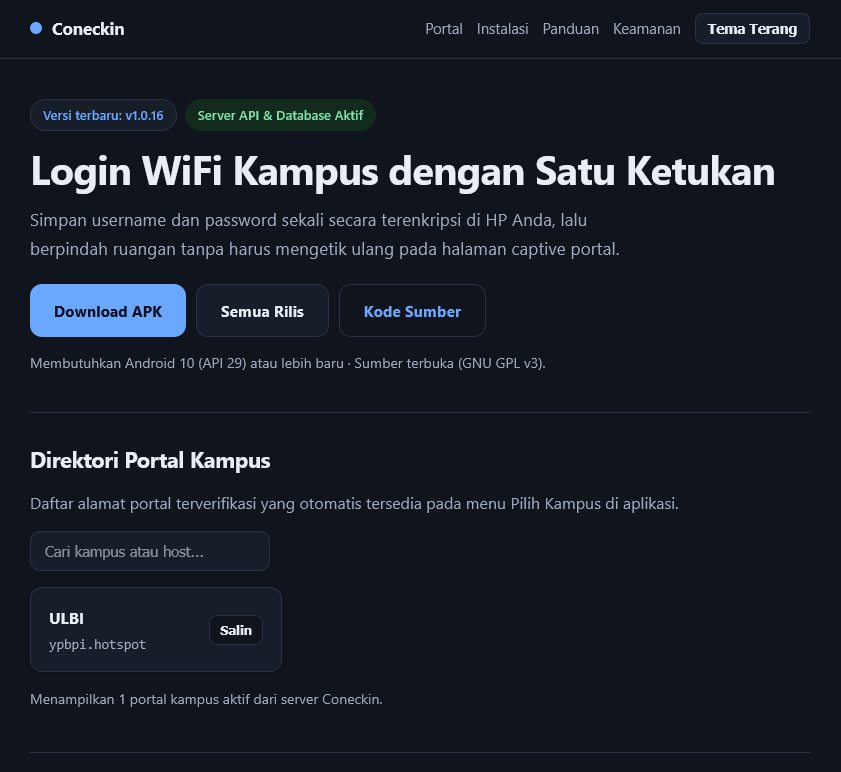
\includegraphics[width=0.92\textwidth]{images/landing-page-live.png}
%   \caption{Tampilan Landing Page \texttt{coneckin.github.io} terhubung aktif dengan API Alwaysdata.}
%   \label{fig:landing-live}
% \end{figure}

\chapter{Penutup}

\section{Kesimpulan}
Berdasarkan hasil pengembangan, pengujian, dan verifikasi produksi ekosistem Coneckin pada Proyek 2 ini, dapat disimpulkan beberapa hal utama:
\begin{enumerate}[leftmargin=*]
  \item Arsitektur \textit{Hybrid CRUD} telah berhasil dilengkapi secara menyeluruh. Di sisi perangkat Android, fitur \textit{Ubah Akun}, validasi duplikasi, ekspor/impor cadangan, serta penguatan keamanan akses (PIN berbasis \texttt{PBKDF2WithHmacSHA256} dengan \textit{lockout}, fitur \textit{Lupa PIN}, verifikasi per sesi, \texttt{BIOMETRIC\_STRONG}, dan minifikasi R8 menghasilkan APK 2,25~MB) melengkapi operasi CRUD lokal di atas enkripsi AES-256 GCM (\texttt{AndroidKeyStore}). Di sisi server, endpoint CRUD penuh untuk koleksi \texttt{portals}, \texttt{app\_config}, dan \texttt{reports} pada basis data \texttt{coneckin\_db} telah beroperasi di Alwaysdata dengan perlindungan autentikasi token admin berbasis SHA-256 \texttt{timingSafeEqual}.
  \item Penjaminan mutu berbasis pengujian otomatis mencapai 140 skenario lulus, terdiri atas 90 \textit{unit test} JVM Android dengan \textit{line coverage} 97,02\% (358/369 baris pada 37 kelas logika), 11 \textit{instrumented test} perangkat Android untuk \texttt{CryptoManager} dan \texttt{AccountStore}, serta 39 pengujian server Express dengan \textit{line coverage} 96,53\%. Ambang \textit{coverage} minimal 80\% telah ditegakkan otomatis pada pipeline CI/CD GitHub Actions sebelum rilis APK/AAB diterbitkan.
  \item \textit{Landing page} berbasis konvensi modular Croot.js pada \url{https://coneckin.github.io/} telah aktif di GitHub Pages dan terintegrasi langsung dengan API produksi \url{https://panlink.alwaysdata.net} (status \texttt{ok: true, db: true}) serta rilis APK terbaru.
\end{enumerate}

\section{Saran}
Untuk pengembangan ekosistem Coneckin selanjutnya, beberapa hal yang disarankan antara lain:
\begin{enumerate}[leftmargin=*]
  \item Menambahkan antarmuka web panel admin sederhana yang memanfaatkan endpoint CRUD berotorisasi \texttt{ADMIN\_TOKEN} untuk memverifikasi usulan portal kampus baru dan memantau ringkasan laporan gangguan.
  \item Mengintegrasikan pengujian UI Jetpack Compose tambahan pada \textit{instrumented test} guna memverifikasi interaksi dialog tambah dan ubah akun secara otomatis pada berbagai ukuran layar.
  \item Memperluas dukungan profil portal kampus lain melalui kontribusi direktori terbuka pada repositori Coneckin.
\end{enumerate}


% ---------- Daftar Pustaka ----------
\bibliographystyle{ieeetr}
\addcontentsline{toc}{chapter}{DAFTAR PUSTAKA}
\bibliography{referensi}

% ---------- Lampiran ----------
\chapter*{LAMPIRAN}
\addcontentsline{toc}{chapter}{LAMPIRAN}

\section*{Lampiran A: Tautan Repositori dan Layanan Produksi}
\begin{itemize}[leftmargin=*]
  \item \textbf{Repositori Utama (Android \& Server API):} \url{https://github.com/coneckin/coneckin}
  \item \textbf{Landing Page Panduan (Croot.js):} \url{https://coneckin.github.io/}
  \item \textbf{Endpoint Kesehatan API Produksi:} \url{https://panlink.alwaysdata.net/health}
  \item \textbf{Paket Rilis APK Terbaru:} \url{https://github.com/coneckin/coneckin/releases/latest/download/coneckin.apk}
\end{itemize}

\section*{Lampiran B: Rincian Code Coverage Logika Non-UI Android (JaCoCo)}
Berikut adalah rincian cakupan baris dari eksekusi task \texttt{verifyLogicCoverage} pada seluruh 37 kelas logika inti Android (total 358/369 baris atau 97,02\%):

\begin{table}[H]
\centering
\caption{Rincian Line Coverage Modul Logika Non-UI Coneckin (JaCoCo)}
\label{tab:jacoco-detail-lampiran}
\small
\begin{tabular}{@{}p{5.8cm}ccc@{}}
\toprule
\textbf{Kelompok / Kelas Logika} & \textbf{Baris Tercakup} & \textbf{Total Baris} & \textbf{Cakupan} \\
\midrule
\texttt{PinManager} \& \texttt{PinCheck.*} (Keamanan PIN) & 68 & 68 & 100,0\% \\
\texttt{ModelsKt}, \texttt{Account}, \texttt{Portal}, \texttt{AppData}, \texttt{InputCheck.*}, \texttt{EditInputCheck.*} & 103 & 103 & 100,0\% \\
\texttt{AccountRepository} \& \texttt{AppDataJson} & 50 & 50 & 100,0\% \\
\texttt{LoginMappingKt} \& \texttt{LoginResult.*} & 28 & 28 & 100,0\% \\
\texttt{PortalSelectionKt} \& \texttt{PortalPick.*} & 14 & 14 & 100,0\% \\
\texttt{RemoteCacheStore} \& \texttt{DirectoryPortal}, \texttt{RemoteConfig} & 28 & 28 & 100,0\% \\
\texttt{ReporterKt} & 11 & 11 & 100,0\% \\
\texttt{ReportQueue} & 39 & 40 & 97,5\% \\
\texttt{RemoteKt} (termasuk pembungkus HTTP \texttt{Api}) & 17 & 27 & 63,0\% \\
\midrule
\textbf{Total (37 Kelas Logika Non-UI)} & \textbf{358} & \textbf{369} & \textbf{97,02\%} \\
\bottomrule
\end{tabular}
\end{table}

\section*{Lampiran C: Ringkasan Konfigurasi CI/CD (\texttt{release.yml})}
Alur kerja \texttt{.github/workflows/release.yml} pada repositori \texttt{coneckin} memastikan pengujian dan verifikasi ambang \textit{coverage} minimal 80\% dijalankan sebelum membangun biner rilis:
\begin{lstlisting}
- name: Unit test dan coverage
  run: ./gradlew testDebugUnitTest createDebugUnitTestCoverageReport verifyLogicCoverage
- name: Build APK dan AAB
  run: ./gradlew assembleRelease bundleRelease
\end{lstlisting}


\end{document}
